\chapter{Plataforma de desarrollo}
\label{cap:capitulo3}

\begin{flushright}
\begin{minipage}[]{10cm}
\emph{Quizás algún fragmento de libro inspirador...}\\
\end{minipage}\\

Autor, \textit{Título}\\
\end{flushright}

\vspace{1cm}

En este capítulo se definen tanto la infraestructura utilizada como los métodos, tanto a nivel software como hardware, que se han utilizado para desarrollar este trabajo.\\

\section{Infraestructura hardware}
\label{sec:hw}
Para este trabajo se ha utilizado la Raspberry Pi 4b+ con su respectivo sistema operativo Raspbian. Junto a ella, se han utilizado una serie de sensores como la PiCam, que es la cámara de Raspberry, una cámara térmica, sensores de temperatura, humedad, calidad del aire o medición del nivel de agua. Para conectar de forma cómoda todos estos sensores se ha utilizado una protoboard junto con los cables dupont necesarios para la correcta instalación de dichos sensores.\\
Para conseguir que todo funcione adecuadamente, se ha utilizado la infraestructura software descrita a continuación.\\
 
\section{Lenguaje python}
\label{sec:python}
Python \footnote{\url{https://www.python.org}} es un lenguaje de alto nivel de programación, interpretado y orientado a objetos cuya filosofía hace hincapié en la legibilidad de su código y por ello su sintaxis es sencilla. Utiliza módulos y librerías como TensorFlow para aplicaciones en Machine Learning, Pandas para análisis de datos, Flask para aplicaciones web o SQLAlchemy para comunicación entre bases de datos y programas, entre otros. Esto facilita la reusabilidad de código y la programación modulada. No requiere del proceso de compilación, lo que lo convierte en un lenguaje muy rápido en el ciclo de edición, prueba y depuración.\\
Actualmente es el lenguaje de programación más usado en el mundo según la calificación de la empresa TIOBE\footnote{\url{https://www.tiobe.com/tiobe-index/}} debido a las características anteriores, formando una gran comunidad. Además, también es el más popular en el ámbito del Machine Learning. Algunas de las aplicaciones que usan Python son Google, Netflix, Dropbox o Spotify.\\

La decisión de usar Python para el desarrollo de este TFG ha sido, además de que el autor está familiarizado con el lenguaje, por las numerosas librerías útiles para este proyecto adaptadas a Raspberry que Python posee.\\
En este trabajo, Python se utiliza para la lectura de los sensores de forma concurrente, para la creación de los dos servidores web que tiene tanto la PiCamera como la cámara térmica con Flask y para el reconocimiento de lo ratones a través de la librería TensorFlow Lite.\\

\section{TensorFlow Lite}
\label{sec:tensor}
TensorFlow Lite \footnote{\url{https://www.tensorflow.org/lite/}} es una variación de TensorFlow adaptada a dispositivos como teléfonos móviles con sistemas operativos como Android o IOS, microcontroladores o dispositivos embebidos como Raspberry. Es una plataforma de código abierto y multiplataforma que entrena un modelo para la posterior clasificación o reconocimiento de imágenes, entre otros.\\
Las características que hacen que pueda utilizarse en este tipo de dispositivos son ligereza, ya que estos dispositivos tienen límite tanto en el almacenamiento como sobretodo en la capacidad de cómputo, baja latencia dado a que las inferencias se realizan en el dispositivo y no en un servidor externo, seguridad ya que el modelo viene implementado en el propio dispositivo o consumo de energía óptimo dado a que no es necesario que el dispositivo esté conectado a la red, que consume mucha energía.\\

El uso de TensorFlow Lite ha sido, en primer lugar, para la creación y entrenamiento de un modelo capaz de detectar ratones en una imagen, basándose en un dataset de 60 imágenes. En segundo lugar, para la detección de ratones en cualquier imagen o vídeo, siendo capaz de detectar el número de ratones o el lugar en el que se encuentra cada uno. Para conseguir esta detección a tiempo real del vídeo grabado por la cámara es requerido el uso de otra librería llamada OpenCV.\\
\begin{figure} [h!]
  \begin{center}
    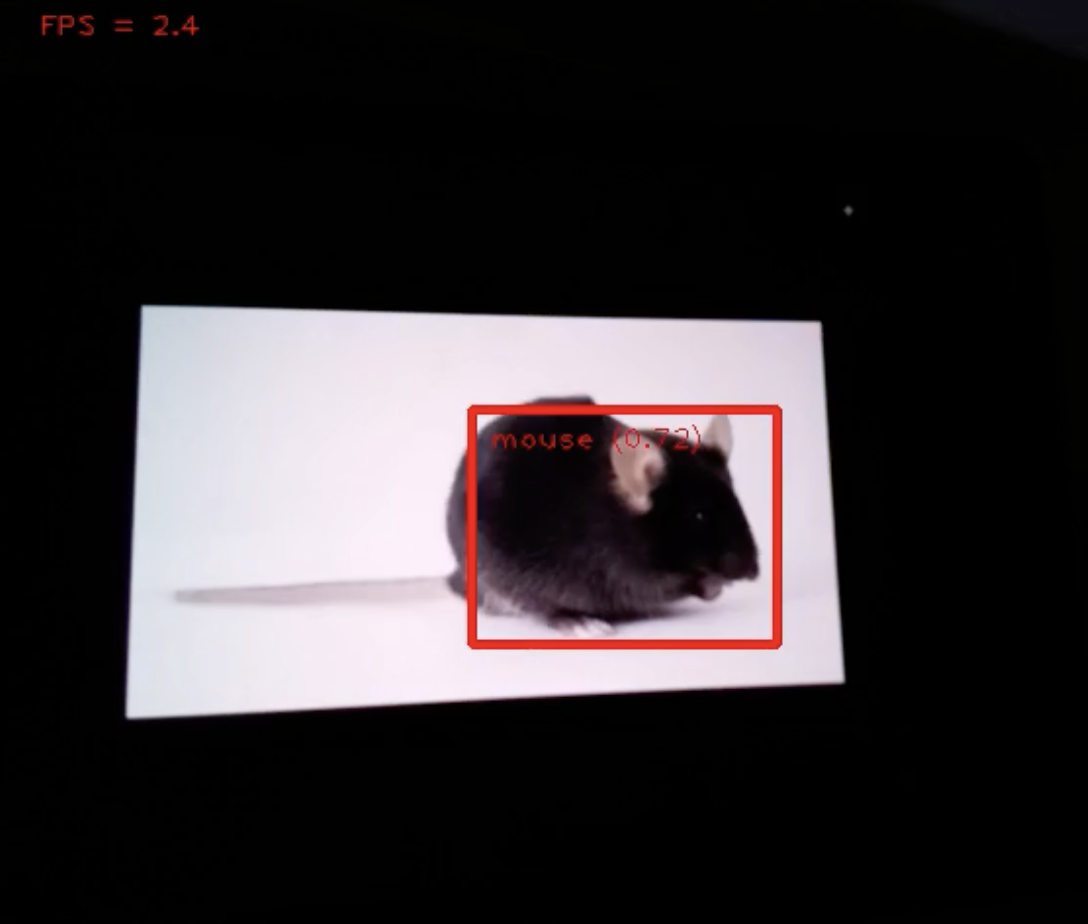
\includegraphics[width=8cm]{figs/raton-detectado}
  \end{center}
  \caption{Detección de ratones en una imagen usando TensorFlow Lite.}
  \label{fig:tesla}
\end{figure}\\

\section{OpenCV}
\label{sec:opencv}
OpenCV \footnote{\url{https://opencv.org}} (Open Source Computer Vision Library) es una librería de software de visión computacional y machine learning de código abierto. Es ampliamente usada en todo el mundo debido al soporte multiplataforma que ofrece para Windows, Linux, MacOS y Android, además de ofrecer interfaz en diferentes lenguajes como Python, Java, C++ y MATLAB.\\
Compuesto por más de 2500 algoritmos, OpenCV está especializado en la visión computacional y en algoritmos de aprendizaje, permitiendo poder hacer cosas como el reconocimiento de rostros, la identificación o clasificación de objetos, la extracción de modelos 3D, el rastreo de los movimientos que hay en cámara, mejorar la calidad de las imágenes, el filtrado de color, la detección de bordes, o las eliminación de los ojos rojos de las fotos.\\
El uso de OpenCV en este trabajo ha permitido la manipulación de los vídeos grabados por las cámaras en tiempo real, de manera que se ha podido integrar en él la fecha y hora del momento, así como poder guardar los vídeos cuando el usuario lo solicite. Debido a su amplio uso y su multitud de librerías, es posible mostrar los vídeos de ambas cámaras en el servidor web sin problema gracias al fácil uso que tiene con Flask.\\
\begin{figure}[h!]
  \begin{center}
    \subfigure[Imagen original]{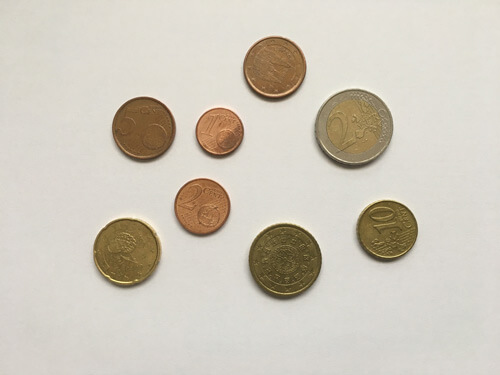
\includegraphics[width=47mm]{figs/monedas}}\hspace{8mm}
    \subfigure[Escala de grises y filtrado de ruido]{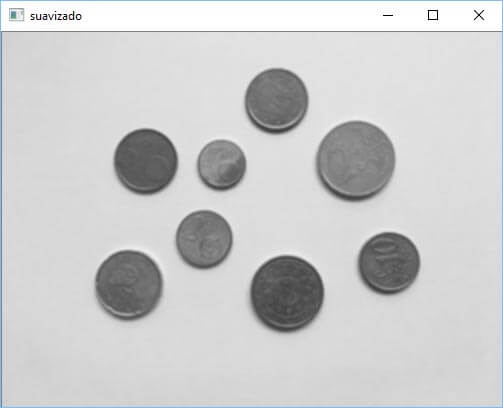
\includegraphics[width=45mm]{figs/suavizado}}\hspace{8mm}
    \subfigure[Detector de bordes]{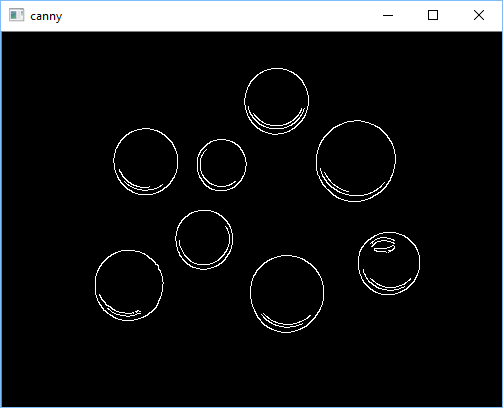
\includegraphics[width=45mm]{figs/detector-bordes}}\hspace{8mm}
    \subfigure[Detector de contornos]{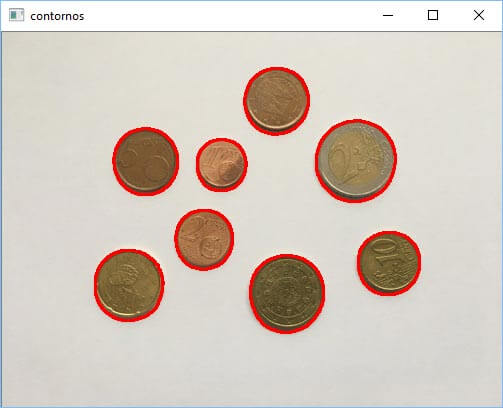
\includegraphics[width=45mm]{figs/contornos}}
  \end{center}
\caption{Ejemplo de detección de bordes con OpenCV.} \label{fig:ej-opencv}
\end{figure}
%imagenes obtenidas de https://programarfacil.com/blog/vision-artificial/detector-de-bordes-canny-opencv/
\section{Flask}
\label{sec:flask}
Flask \footnote{\url{https://flask.palletsprojects.com/en/2.1.x/}} es un \textit{microframework} web escrito en Python. Esto significa que ofrece al usuario herramientas y librerías para crear una aplicación web, y al ser minimalista, no requiere de otras dependencias para realizar las cosas básicas. Ofrece una serie de extensiones que permiten dotar de más características a la aplicación, como autenticación o manejo a través de comandos entre otros.\\
Se compone de dos partes; los \textit{templates}, que están escritos en HTML e indican la organización y diseño que tendrá cada página al ser visualizada y la parte de código en python que indica las rutas de cada página y las funciones de cada ruta, es el fichero que se ejecuta para crear el servidor, y por defecto éste se crea en el puerto 5000, aunque se puede modificar.\\

Para este proyecto se ha utilizado Flask para crear los dos servidores web de las cámaras. Se ha preferido Flask frente a Django \footnote{\url{https://www.djangoproject.com }}, que es el más conocido para el uso con Python, debido a que es más sencillo de utilizar y de aprender. En estos servidores, después de haber realizado el \textit{login} o el registro con el \textit{plugin} flask-login, se accede a la visualización de cada cámara. Además, en el caso de la cámara normal, usando Flask se ha integrado un botón que permite empezar o parar la grabación del vídeo. \\
\begin{figure}[h!]
  \begin{center}
    \subfigure[Servidor para la cámara térmica]{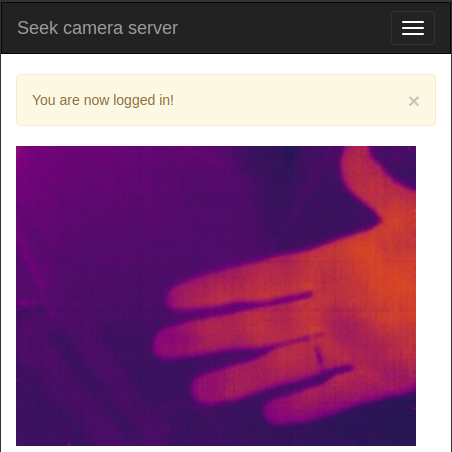
\includegraphics[width=55mm]{figs/termica-server}}\hspace{8mm}
    \subfigure[Servidor para la PiCamera]{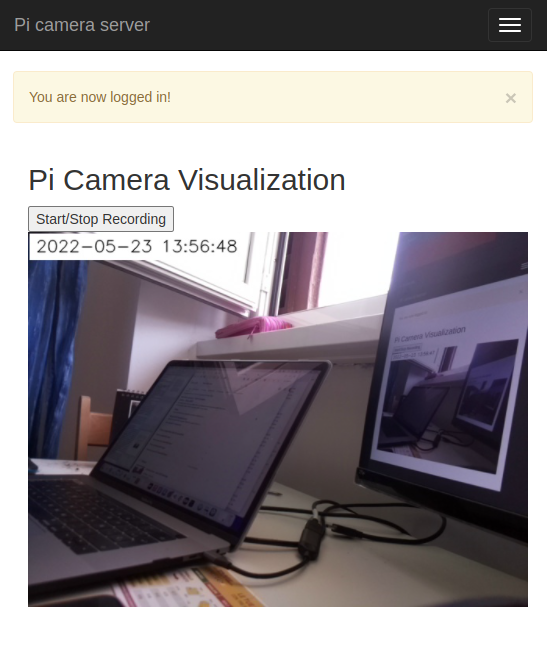
\includegraphics[width=50mm]{figs/picam-server}}
  \end{center}
\caption{Muestra de los dos servidores del trabajo usando Flask.} \label{fig:servers}
\end{figure}

\section{Node-Red}
\label{sec:nodered}
Node-Red \footnote{url{https://nodered.org}} es una herramienta de programación creada por IBM y escrita en JavaScript que permite conectar dispositivos hardware y servicios en línea. Muestra de manera visual las relaciones de los distintos componentes mediante nodos en un panel, mostrando gráficamente el flujo de la información, además de que es un entorno de ejecución ligero que está basado en Node.js, haciéndolo ideal para ejecutarse en hardware de bajo coste como la Raspberry.\\
Está compuesto por dos partes principales. Una de ellas es la edición de flujo desde navegador, donde muestra los nodos disponibles en el margen izquierdo así como la disposición y conexión del flujo que siguen los nodos seleccionados en la pantalla central. La otra parte, es la llamada \textit{dashboard}, que muestra la interfaz de usuario en base al flujo de los nodos de la parte previamente comentada.\\
Node-Red tiene una amplia variedad de nodos, permitiendo conexiones MQTT, UDP, TCP, la interacción directa con los pines de Raspberry, la conexión con twitter o el correo electrónico, la creación de ficheros tipo csv, xml o json o la ejecución de ficheros ya existentes en la computadora. También permite la creación de funciones directamente en el flujo de nodos, teniendo en cuenta que tienen que ser escritas en JavaScript. Pueden crearse nuevos nodos para agregar nuevas capacidades gracias a los más de 225000 módulos que hay en el repositorio de paquetes.\\
Los flujos de datos se pueden importar o exportar con ficheros JSON, permitiendo compartirlos con cualquier persona. La página de Node-Red tiene una librería de flujos que han creado otros usuarios, teniendo así acceso a ellos para utilizarlos como base en otros proyectos.\\
\begin{figure} [h!]
  \begin{center}
    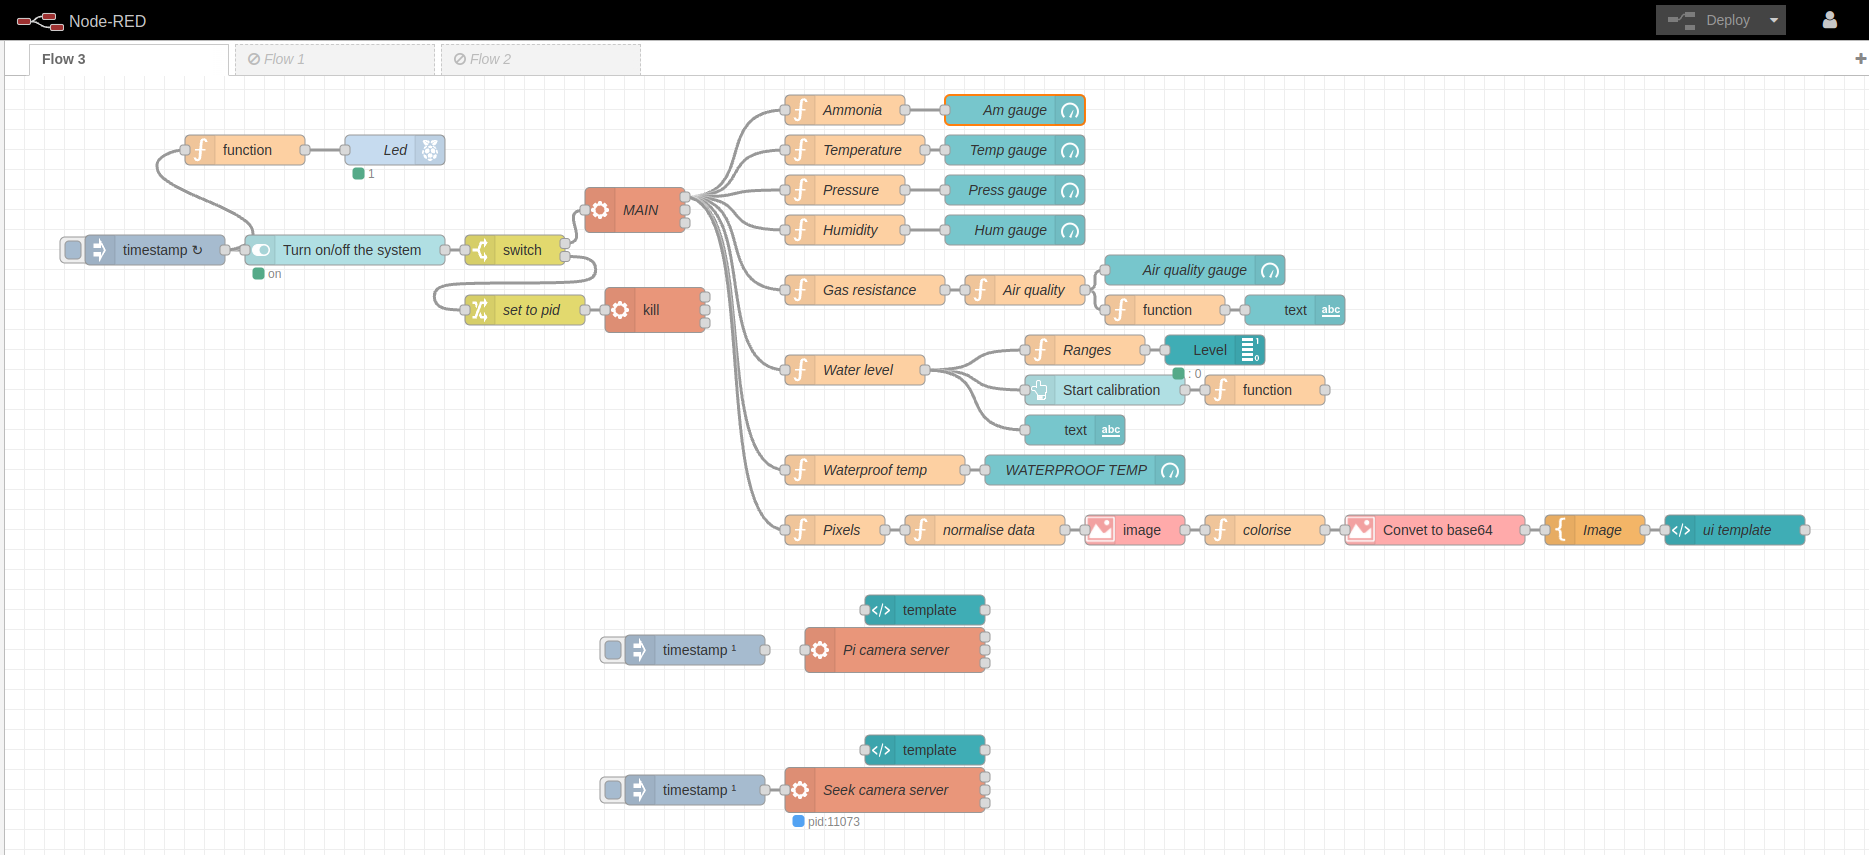
\includegraphics[width=15cm]{figs/flujo}
  \end{center}
  \caption{Flujo del proyecto en Node-Red.}
  \label{fig:flow}
\end{figure}
\newpage
Para el desarrollo de este TFG, Node-Red ha tenido un papel muy importante. Además de tener una gran comunidad que permite la resolución rápida de cualquier duda, ha permitido la creación de la interfaz de usuario sin problema, donde se muestran las mediciones de cada sensor, los dos servidores web de las cámaras y los \textit{widgets} necesarios que permiten al usuario interactuar con la interfaz de una manera sencilla para obtener toda la información.\\
\begin{figure} [h!]
  \begin{center}
    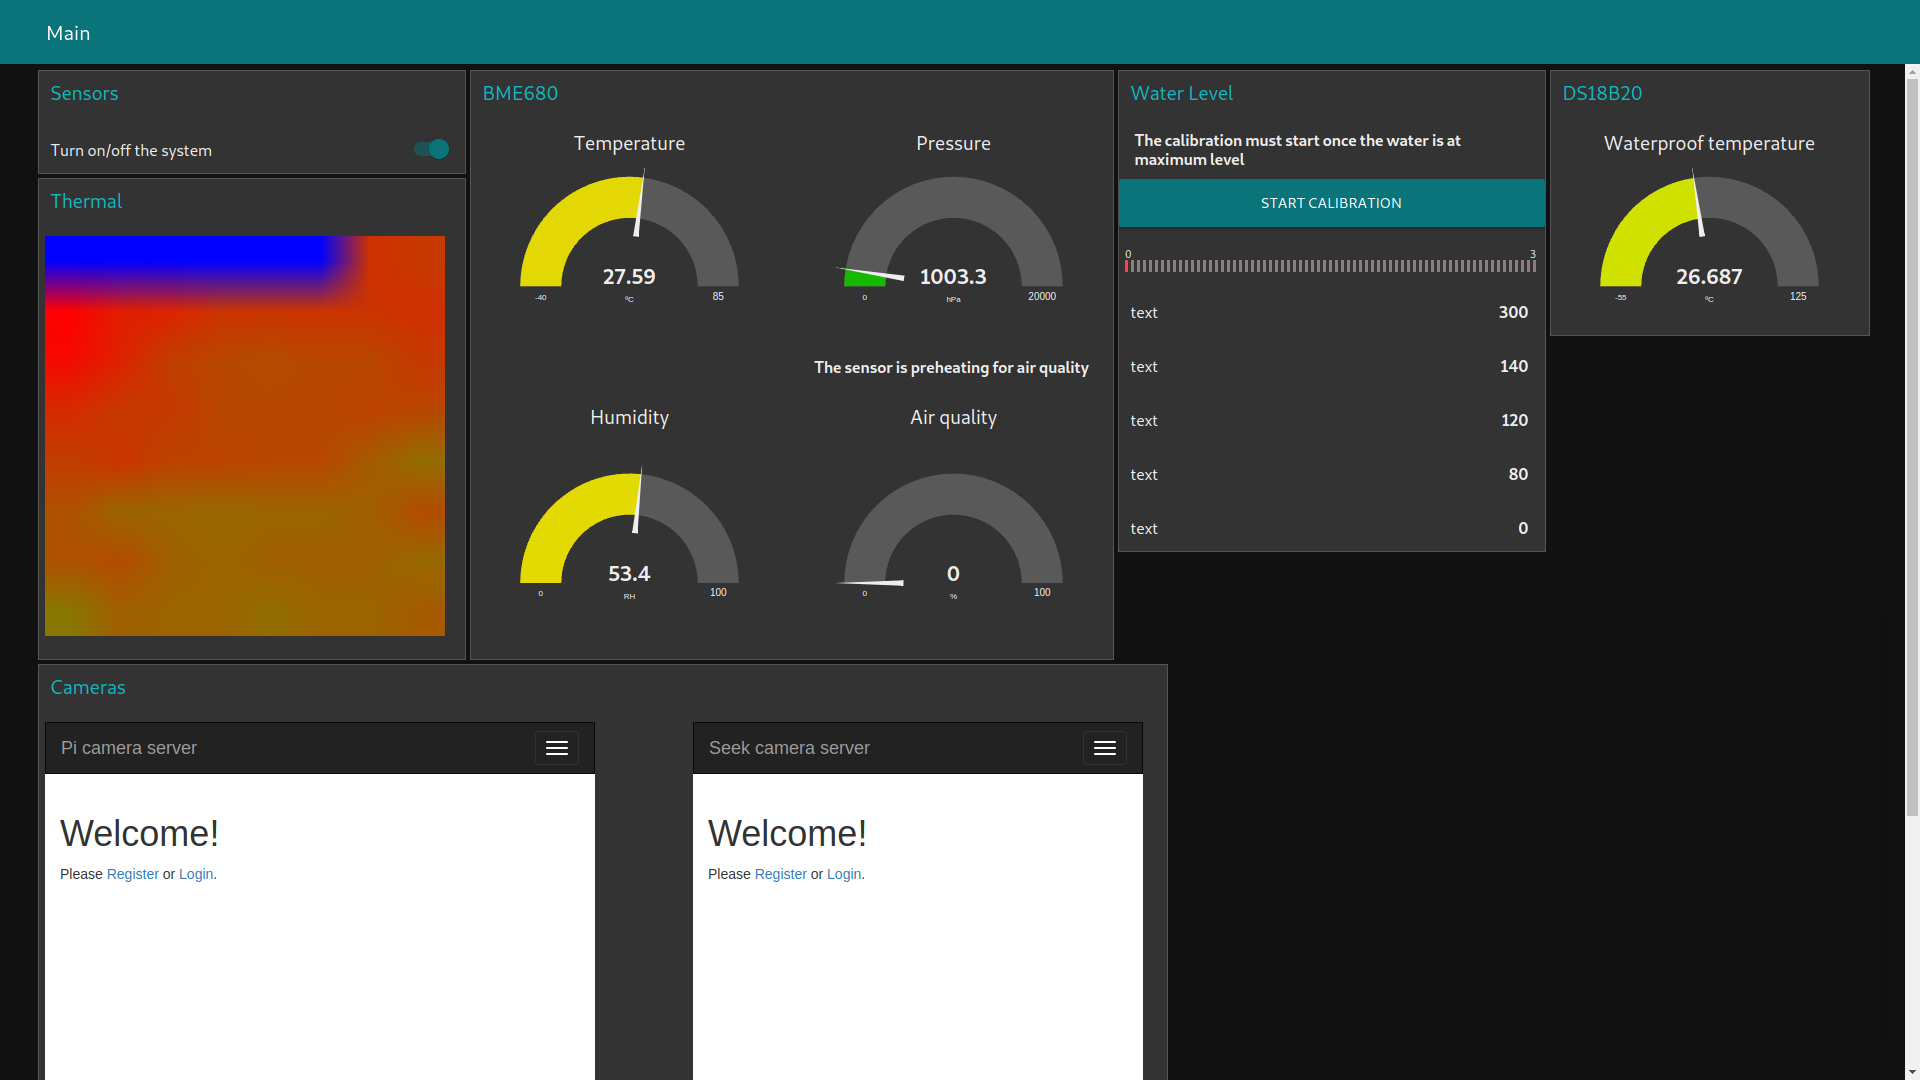
\includegraphics[width=15cm]{figs/interfaz}
  \end{center}
  \caption{Muestra del uso de Node-Red en el trabajo.}
  \label{fig:node-imagenes}
\end{figure}

